% 编译：xelatex -interaction=nonstopmode -halt-on-error -output-directory=figures paper/figures/q1_methodology_flowchart.tex
% 插图：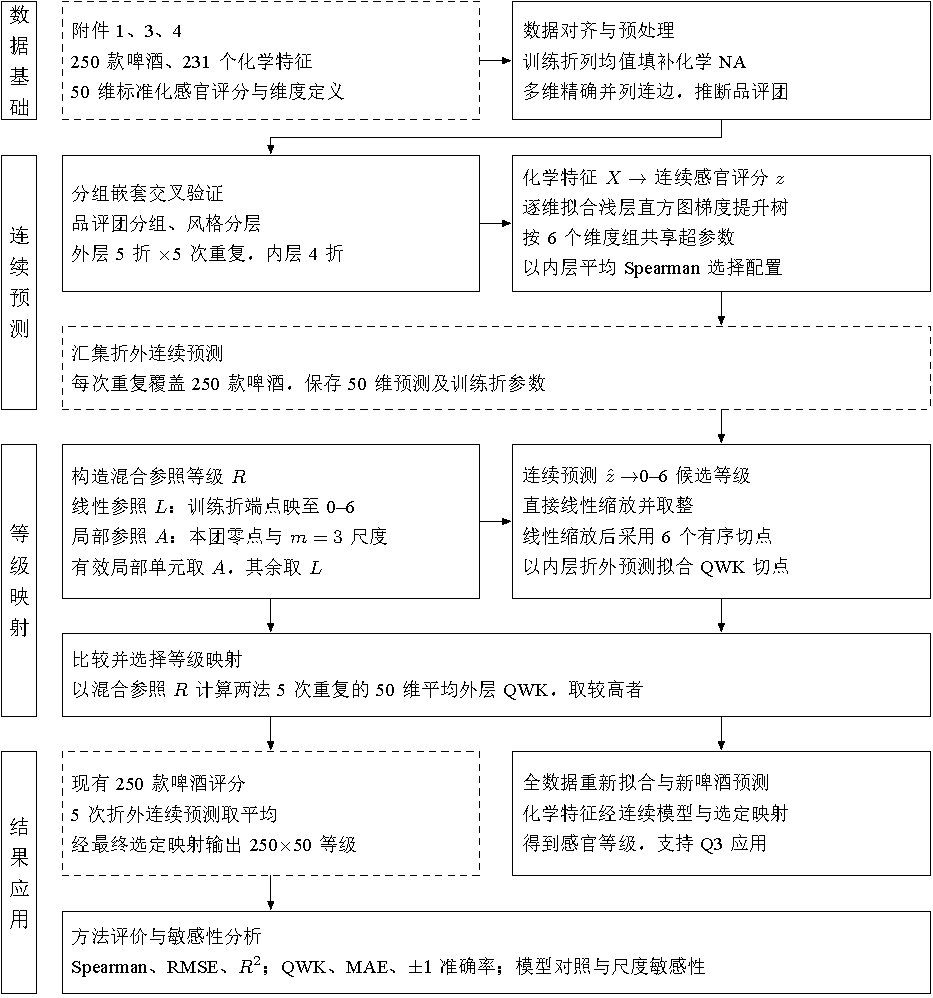
\includegraphics[width=\linewidth]{q1_methodology_flowchart.pdf}
\documentclass[tikz,border=0pt]{standalone}
\usepackage[UTF8,fontset=windows]{ctex}
\usepackage{amsmath}
\usepackage{fontspec}
\usetikzlibrary{arrows.meta,calc}
\setmainfont{Times New Roman}
\begin{document}
\begin{tikzpicture}[x=1mm,y=-1mm,>=Latex,
  line width=0.45pt,
  box/.style={draw,rectangle,anchor=north west,inner sep=1.6mm,outer sep=0pt,align=left,font=\songti\fontsize{9.2}{11.2}\selectfont},
  side/.style={draw,rectangle,anchor=north west,inner sep=0pt,outer sep=0pt,text width=5.8mm,align=center,font=\songti\fontsize{10}{11.5}\selectfont},
  edge/.style={->,line width=0.45pt},
  small/.style={font=\songti\fontsize{8.5}{12}\selectfont,fill=white,inner sep=0.5mm}]
\path[use as bounding box] (0,0) rectangle (158,169);

% 数据基础：输入与预处理。
\node[side,minimum height=20mm] at (0.3,0.3) {数\\据\\基\\础};
\node[box,dashed,text width=67.5mm,minimum height=20mm] (data) at (10.5,0.3) {附件1、3、4\\250款啤酒、231个化学特征\\50维标准化感官评分与维度定义};
\node[box,text width=67.5mm,minimum height=20mm] (prep) at (86.8,0.3) {数据对齐与预处理\\训练折列均值填补化学NA\\多维精确并列连边，推断品评团};
\draw[edge] (data.east) -- (prep.west);

% 连续预测：分组调参与逐维回归。
\node[side,minimum height=43mm] at (0.3,26.3) {连\\续\\预\\测};
\node[box,text width=67.5mm,minimum height=23mm] (cv) at (10.5,26.3) {分组嵌套交叉验证\\品评团分组、风格分层\\外层5折$\times$5次重复，内层4折};
\node[box,text width=67.5mm,minimum height=23mm] (model) at (86.8,26.3) {化学特征$X\to$连续感官评分$z$\\逐维拟合浅层直方图梯度提升树\\按6个维度组共享超参数\\以内层平均Spearman选择配置};
\draw[edge] (prep.south) -- ++(0,3) -| (cv.north);
\draw[edge] (cv.east) -- (model.west);
\node[box,dashed,text width=143.8mm,minimum height=14mm] (oof) at (10.5,55.3) {汇集折外连续预测\\每次重复覆盖250款啤酒，保存50维预测及训练折参数};
\draw[edge] (model.south) -- (model.south |- oof.north);

% 等级映射：参照构造与候选映射并列。
\node[side,minimum height=46mm] at (0.3,75.3) {等\\级\\映\\射};
\node[box,text width=67.5mm,minimum height=26mm] (reference) at (10.5,75.3) {构造混合参照等级$R$\\线性参照$L$：训练折端点映至0--6\\局部参照$A$：本团零点与$m=3$尺度\\有效局部单元取$A$，其余取$L$};
\node[box,text width=67.5mm,minimum height=26mm] (mapping) at (86.8,75.3) {连续预测$\hat z\to$0--6候选等级\\直接线性缩放并取整\\线性缩放后采用6个有序切点\\以内层折外预测拟合QWK切点};
\draw[edge] (oof.south -| mapping.north) -- (mapping.north);
\draw[edge] (reference.east) -- (mapping.west);
\node[box,text width=143.8mm,minimum height=14mm] (select) at (10.5,107.3) {比较并选择等级映射\\以混合参照$R$计算两法5次重复的50维平均外层QWK，取较高者};
\draw[edge] (reference.south) -- (reference.south |- select.north);
\draw[edge] (mapping.south) -- (mapping.south |- select.north);

% 结果应用：现有样本使用折外预测，新样本使用全数据模型。
\node[side,minimum height=41mm] at (0.3,127.3) {结\\果\\应\\用};
\node[box,dashed,text width=67.5mm,minimum height=21mm] (scores) at (10.5,127.3) {现有250款啤酒评分\\5次折外连续预测取平均\\经最终选定映射输出250$\times$50等级};
\node[box,text width=67.5mm,minimum height=21mm] (new) at (86.8,127.3) {全数据重新拟合与新啤酒预测\\化学特征经连续模型与选定映射\\得到感官等级，支持Q3应用};
\draw[edge] (select.south -| scores.north) -- (scores.north);
\draw[edge] (select.south -| new.north) -- (new.north);
\node[box,text width=143.8mm,minimum height=14mm] (metrics) at (10.5,154.3) {方法评价与敏感性分析\\Spearman、RMSE、$R^2$；QWK、MAE、$\pm1$准确率；模型对照与尺度敏感性};
\draw[edge] (scores.south) -- (scores.south |- metrics.north);
\end{tikzpicture}
\end{document}
